%\documentclass[pdftex]{beamer}
%\documentclass[notes=show]{beamer}
%\documentclass[xcolor=dvipsnames]{beamer}
\documentclass[notes=show,beamer,compress]{beamer}

\usepackage{amssymb}
\usepackage{latexsym}
\usepackage{amsfonts}
\usepackage{amsmath}
\usepackage[absolute,overlay]{textpos}
\usepackage[english]{babel}
\usepackage[latin1]{inputenc}
%\usepackage{times}
\usepackage[T1]{fontenc}
\usepackage{tikz}
\usetikzlibrary{arrows,positioning} 
\usepackage{graphicx}
\usepackage{bigstrut}
\usepackage{bbm}
\usepackage{mathrsfs}
\usepackage{epsfig}
\usepackage{array}
%\usepackage{natbib}

\tikzstyle{arrow} = [thick,->,>=stealth]

\mode<presentation> {
	%\usetheme[left,width=1.7cm]{Berkeley}
	%\usetheme{default}
	\usetheme{Boadilla}
	\usecolortheme[RGB={103,102,204}]{structure}
	%\usecolortheme{dove}
	\useoutertheme{infolines}
	\setbeamercovered{transparent}
}

%\renewcommand{\familydefault}{cmss}
%\renewcommand{\mathrm}{\mathsf}
%\renewcommand{\textrm}{\textsf}
%\usefonttheme{serif}
\newcommand{\X}{{\mathbf{X}}}
\newcommand{\x}{{\mathbf{x}}}
\newcommand{\E}{\mathsf{E}}
\newcommand{\V}{\mathsf{Var}}


%%%%%%%%%%%%%%%%%%%%%%%%%%%%%%%%%%%%%%%%%%%%%%%%%%%%%%%%%%%%%%%%%%%%%%%%%%%%%%
%         Neue Kommandos f�r fette Mathebuchstaben innerhalb von Formeln     %
%%%%%%%%%%%%%%%%%%%%%%%%%%%%%%%%%%%%%%%%%%%%%%%%%%%%%%%%%%%%%%%%%%%%%%%%%%%%%%
\newcommand{\bom}{\boldmath}
\newcommand{\ubom}{\unboldmath}
\newcommand{\mb}{\mathbf}

\newcommand{\fmalpha}{\mbox{\bom${\alpha}$}}               %Fettes alpha
\newcommand{\fmbeta}{\mbox{\bom${\beta}$}}                 %Fettes beta
\newcommand{\fmgamma}{\mbox{\bom${\gamma}$}}               %Fettes gamma
\newcommand{\fmdelta}{\mbox{\bom${\delta}$}}               %Fettes delta
\newcommand{\fmepsilon}{\mbox{\bom${\epsilon}$}}           %Fettes epsilon
\newcommand{\fmvarepsilon}{\mbox{\bom${\varepsilon}$}}     %Fettes varepsilon
\newcommand{\fmzeta}{\mbox{\bom${\zeta}$}}                 %Fettes zeta
\newcommand{\fmeta}{\mbox{\bom${\eta}$}}                   %Fettes eta
\newcommand{\fmta}{\mbox{\bom${\theta}$}}                  %Fettes theta (ta)
\newcommand{\fmvarta}{\mbox{\bom${\vartheta}$}}         	 %Fettes vartheta (ta)
\newcommand{\fmiota}{\mbox{\bom${\iota}$}}                 %Fettes iota
\newcommand{\fmkappa}{\mbox{\bom${\kappa}$}}               %Fettes kappa
\newcommand{\fmla}{\mbox{\bom${\la}$}}                     %Fettes lambda (la)
\newcommand{\fmmu}{\mbox{\bom${\mu}$}}                     %Fettes mu
\newcommand{\fmnu}{\mbox{\bom${\nu}$}}                     %Fettes nu
\newcommand{\fmxi}{\mbox{\bom${\xi}$}}                     %Fettes xi
\newcommand{\fmo}{\mbox{\bom${\o}$}}                       %Fettes o
\newcommand{\fmpi}{\mbox{\bom${\pi}$}}                     %Fettes pi
\newcommand{\fmvarpi}{\mbox{\bom${\varpi}$}}               %Fettes varpi
\newcommand{\fmrho}{\mbox{\bom${\rho}$}}                   %Fettes rho
\newcommand{\fmvarrho}{\mbox{\bom${\varrho}$}}             %Fettes varrho
\newcommand{\fmsigma}{\mbox{\bom${\sigma}$}}               %Fettes sigma
\newcommand{\fmvarsigma}{\mbox{\bom${\varsigma}$}}         %Fettes varsigma
\newcommand{\fmtau}{\mbox{\bom${\tau}$}}                   %Fettes tau
\newcommand{\fmupsilon}{\mbox{\bom${\upsilon}$}}           %Fettes upsilon
\newcommand{\fmphi}{\mbox{\bom${\phi}$}}                   %Fettes phi
\newcommand{\fmvarphi}{\mbox{\bom${\varphi}$}}             %Fettes varphi
\newcommand{\fmchi}{\mbox{\bom${\chi}$}}                   %Fettes chi
\newcommand{\fmpsi}{\mbox{\bom${\psi}$}}                   %Fettes psi
\newcommand{\fmomega}{\mbox{\bom${\omega}$}}               %Fettes omega
\newcommand{\fmimath}{\mbox{\bom${\imath}$}}               %Fettes imath

\newcommand{\fmv}{\mathnormal{v}}               %v
\newcommand{\fmu}{\mathnormal{u}}               %v
\newcommand{\fme}{\mathnormal{e}}               %v


\setbeamercolor{bibliography entry title}{fg=black}
\setbeamercolor{bibliography entry author}{fg=black}
\setbeamercolor{subsection in toc}{fg=structure}
\setbeamercolor{palette primary}{bg=structure, fg=white}
%\setbeamercolor{palette secondary}{bg=structure, fg=black}
%\setbeamercolor{palette tertiary}{bg=structure, fg=black}
\setbeamercolor{caption name}{fg=black} \setbeamersize{text margin
	left=.8cm} \setbeamersize{text margin right=1cm}
\hypersetup{linkbordercolor={1 0 0}} \setbeamertemplate{navigation
	symbols}{} \setbeamertemplate{headline}[default]

\setbeamertemplate{enumerate items}[default]

\newcounter{transfct}
\newcounter{begbs}
\newcounter{endbs}
\title[]{Econometrics 2}
\subtitle{}
\author[Lychagin \& Mu\c{c}o]{Sergey Lychagin}
\institute[CEU]{CEU}
\date{Winter 2020}


\AtBeginSection[] {
	\begin{frame}<handout:0>
	\frametitle{TOC}
	\tableofcontents[currentsection]
\end{frame}
}



\pgfdeclareimage[height=.7cm]{logo}{rgs2}
\logo{\pgfuseimage{logo}}
\begin{document}

\frame{\titlepage}



\begin{frame}
\frametitle{Evaluating Training Programs}
\begin{itemize}
\item What is the causal effect of participating in a training program on future earnings?
\item Government programs for unemployed or disadvantaged workers lacking basic skills
\item Training: counseling, work experience, courses
\item Evaluation strategies
	\begin{itemize}
		\item Experimental evaluations: randomized assignment
		\item Non-experimental methods relying on CIA: simple regression, diff-in-diff, Heckman's correction, propensity score matching.
	\end{itemize}
\item Do these methods find similar results?
\item LaLonde (1986), Dehejia and Wahba JASA (1999)

\end{itemize}
\end{frame}

\begin{frame}
\frametitle{National Supported Work Demonstration}
\begin{itemize}
\item National Supported Work Demonstration (NSW): temporary employment program to help disadvantaged workers lacking basic skills to move in to labor market.
\item Separate programs for males and females (AFDC, mostly single unemployed mothers)
\item Experiment: Random assignment of qualified applicants  to \emph{treatment} groups and \emph{control} groups in 10 sites across the US.
\item Guaranteed 9-18 months job plus counseling.
\item Data: Survey with baseline information 4 follow up interviews.
\item Individual level panel data, male sample $t=1975, ..., 1979$
\item Training participation in $1976 -1977$
\item Baseline period: $1975$, After period: $t=1979$
\item Experimental Results
\end{itemize}
\end{frame}

 \frame{ \frametitle{}
\begin{center}
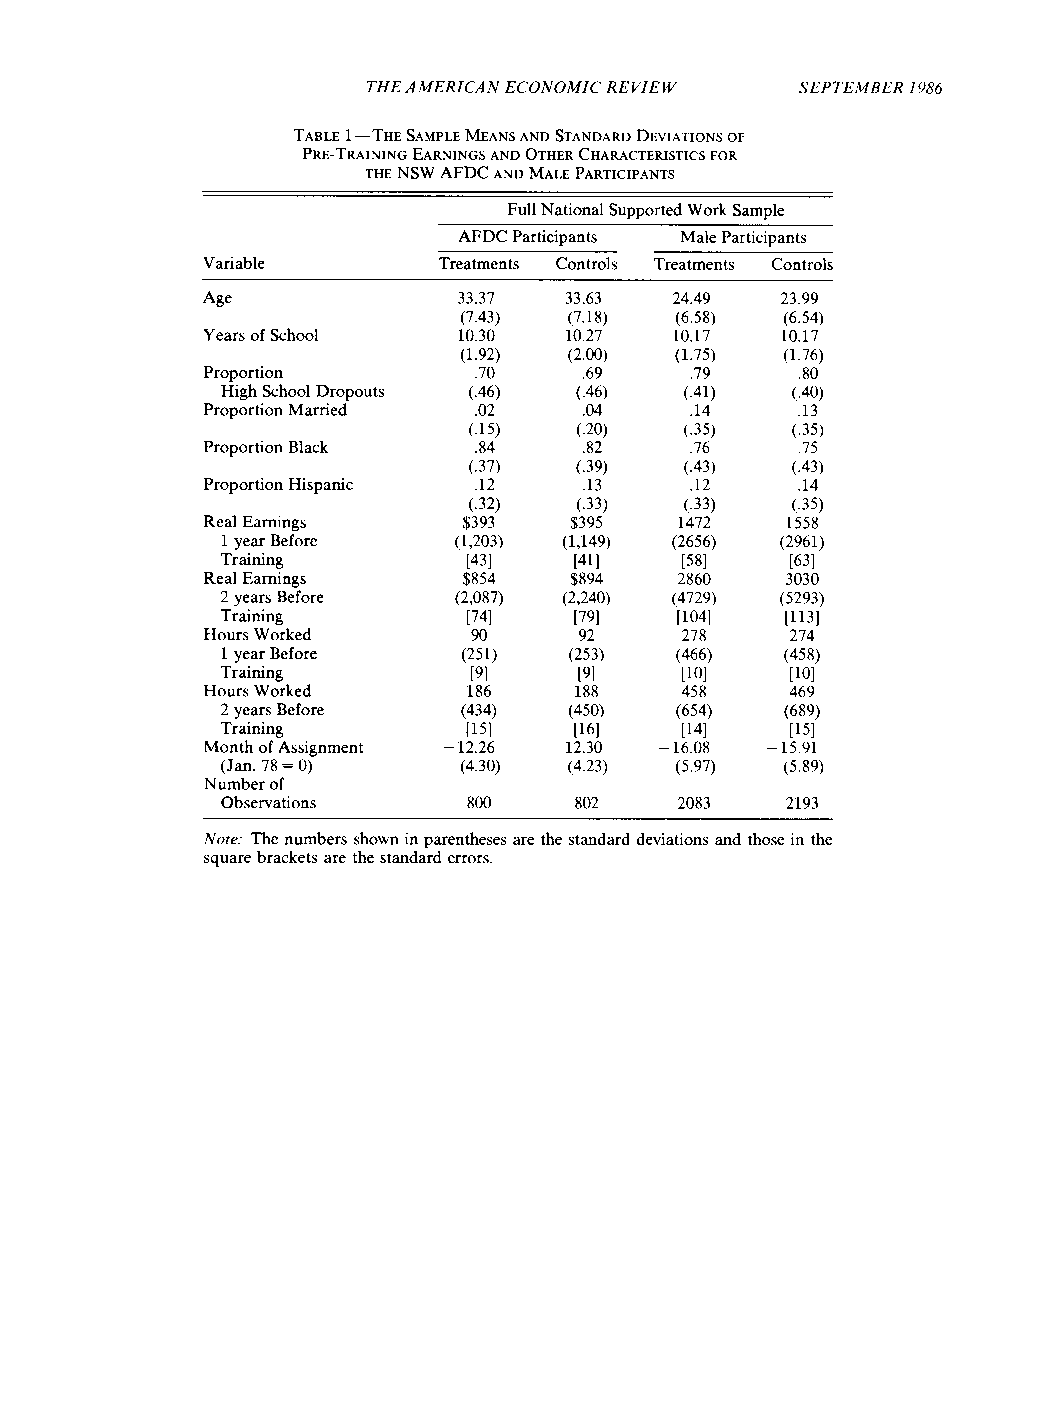
\includegraphics[width=0.80\linewidth]{graphs/lal_tab1.pdf}
\end{center}
 }





\begin{frame}
\frametitle{Non-experimental Evaluation}

Keep observations from the treatment group
\begin{enumerate}
\item Select a control group from publicly available data
\item Choose an econometric model to control for selection into training
\end{enumerate}

Choice of control groups:
\begin{itemize}
\item PSID: nationally representative panel surveys of households
\item PSID-1: male household heads continuously observed 1975 - 1978
\item PSID-2: men not working in spring 1976
\item PSID-3: men not working in spring 1975 and 1976
\item CPS-3: men unemployed in 1976 with income below poverty level in 1975
\end{itemize}
Ideally --- make the control and the treatment group look similar in observables.

\end{frame}


\frame{ \frametitle{}
\begin{center}
	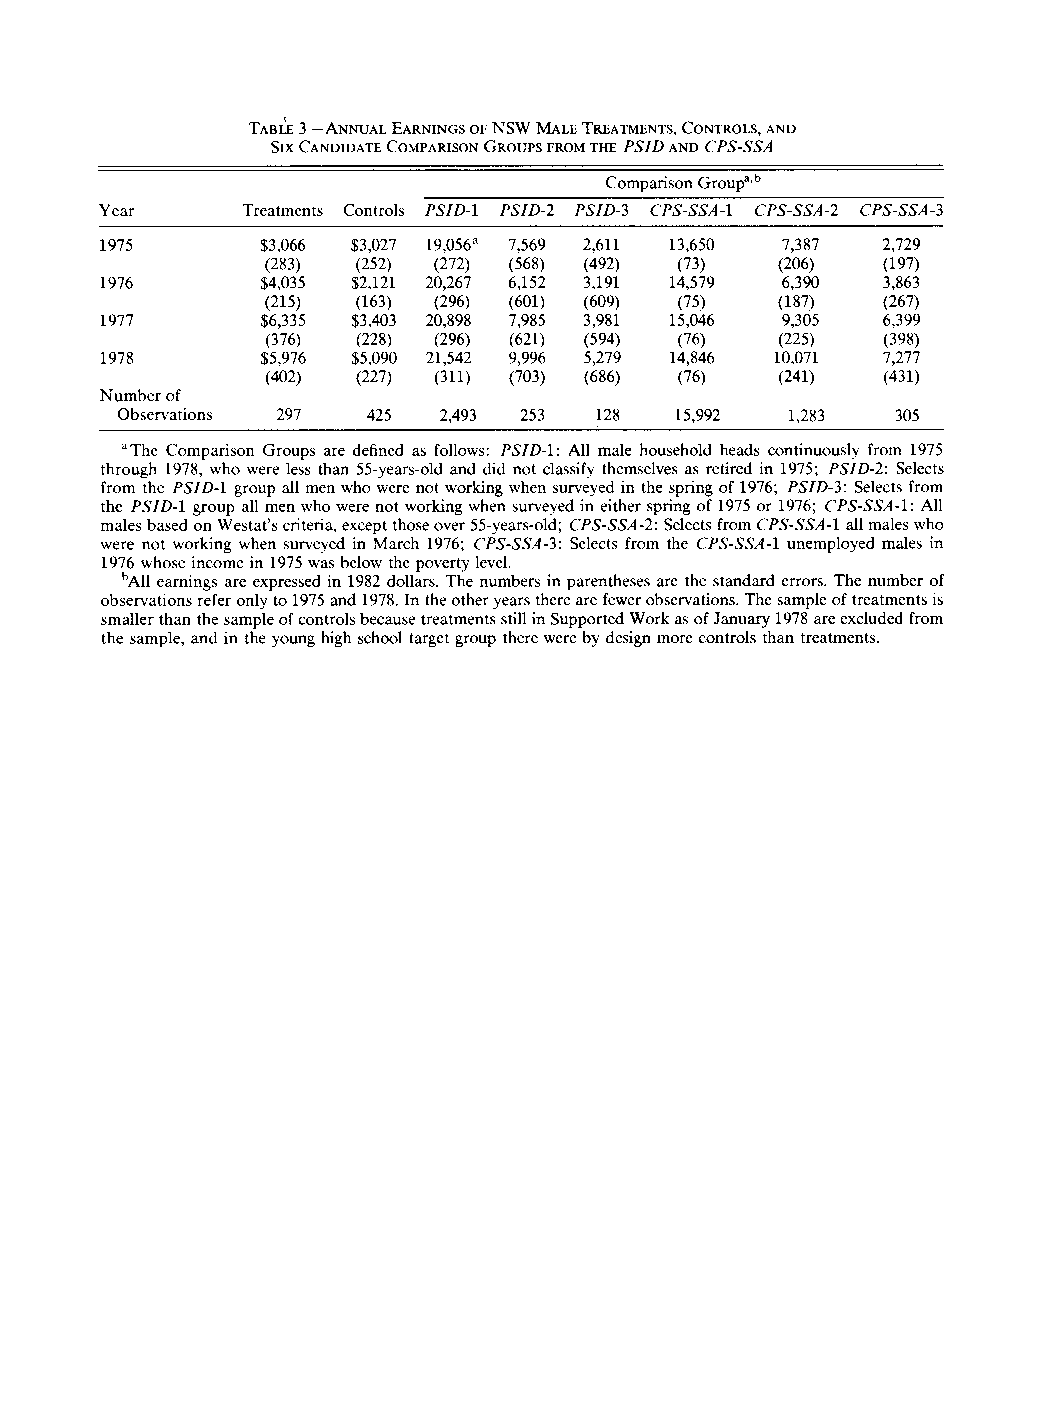
\includegraphics[width=1.0\linewidth]{graphs/lal_tab3.pdf}
\end{center}
 }





\begin{frame}
\frametitle{Econometric Evaluation Methods}
Main threat to identification --- selection on observables and unobservables. Treatment is administered to a very special group!

Regression based methods

\begin{eqnarray*}
	Y_{it}&=& \delta D_i + \beta X_{it} + a_i + b_t + \epsilon_{it} \\
%	d_{is}&=& \gamma_{is}+ \gamma Z_{is}+ \eta_{is} \\
	D_i&=& \left\{ \begin{array}{cc}
                                                1 & \text{if}\;\; \text{treated} \\
                                                0& \text{if}\;\; \text{control}
                                                 \end{array} \right. 
\end{eqnarray*}
	
\begin {itemize}
\item Unadjusted $Y_{it}= \delta D_i +  \epsilon_{it}, \;\;\; t=1978$
\item Adjusted $Y_{it}= \delta D_i +  \beta X_{it}+  \epsilon_{it}, \;\;\; t=1978$
\item FD: $Y_{it}= \delta D_i + \beta X_{it} + a_i + b_t + \epsilon_{it}$,
$t=1975, 1978$ (difference-in-differences)
\item FD controlling for pre-training earnings (``quasi difference'').
\end{itemize}

\end{frame}

\begin{frame}{Female participants (AFDC)}
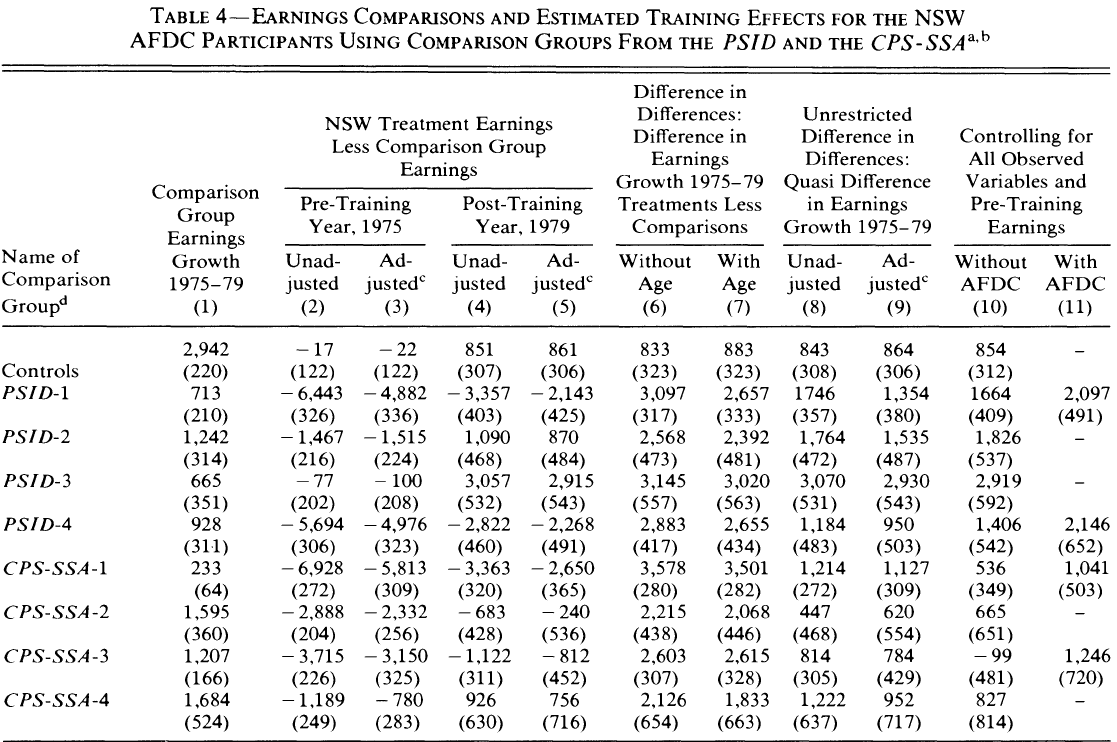
\includegraphics[width=1.0\linewidth]{graphs/lalonde86_4.png}
\end{frame}

\begin{frame}{Female participants (AFDC)}
\begin{itemize}
	\item Columns (2-3): cross-sectional regressions aren't performing well. Selection on unobservables? Rule out (4-5)
	\item Ashenfelter's dip (see Table 1). Simple diff-in-diff is not a good idea. Rule out (6-7).
	\item Specifications (8-11) look okay, but:
		\begin{itemize}
			\item the estimates are sensitive to sample choice
			\item better balance $\to$ smaller sample $\to $ large std. errors
		\end{itemize}
\end{itemize}
\end{frame}

\begin{frame}{Male participants}
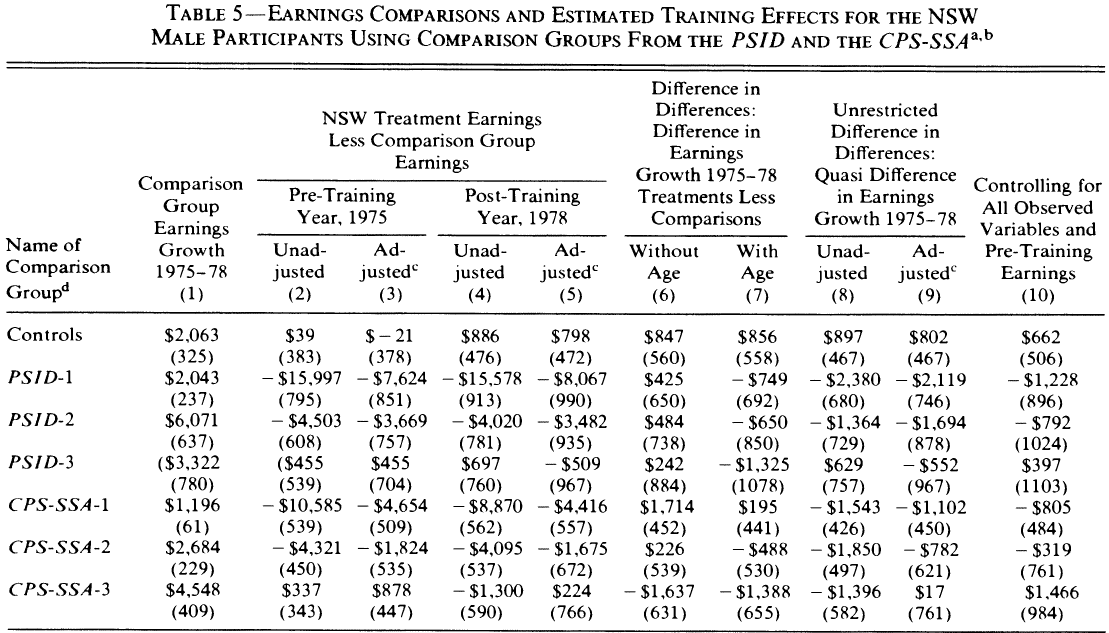
\includegraphics[width=1.0\linewidth]{graphs/lalonde86_5.png}
\end{frame}


\begin{frame}{Heckman correction}

In theory, this takes care of selection on unobservables
\begin{enumerate}
	\item Run probit: $D_i$ on pre-training demographics, $Z_{i}$, compute the correction term (``estimate of expectation''). 
	\item Run earnings post-treatment on controls, $X_i$ and the correction term from step 1.
\end{enumerate}

One extra dimension of modeling choice: exclusion restriction: what controls are included in $Z_i$, but not $X_i$?

\end{frame}


\begin{frame}{}
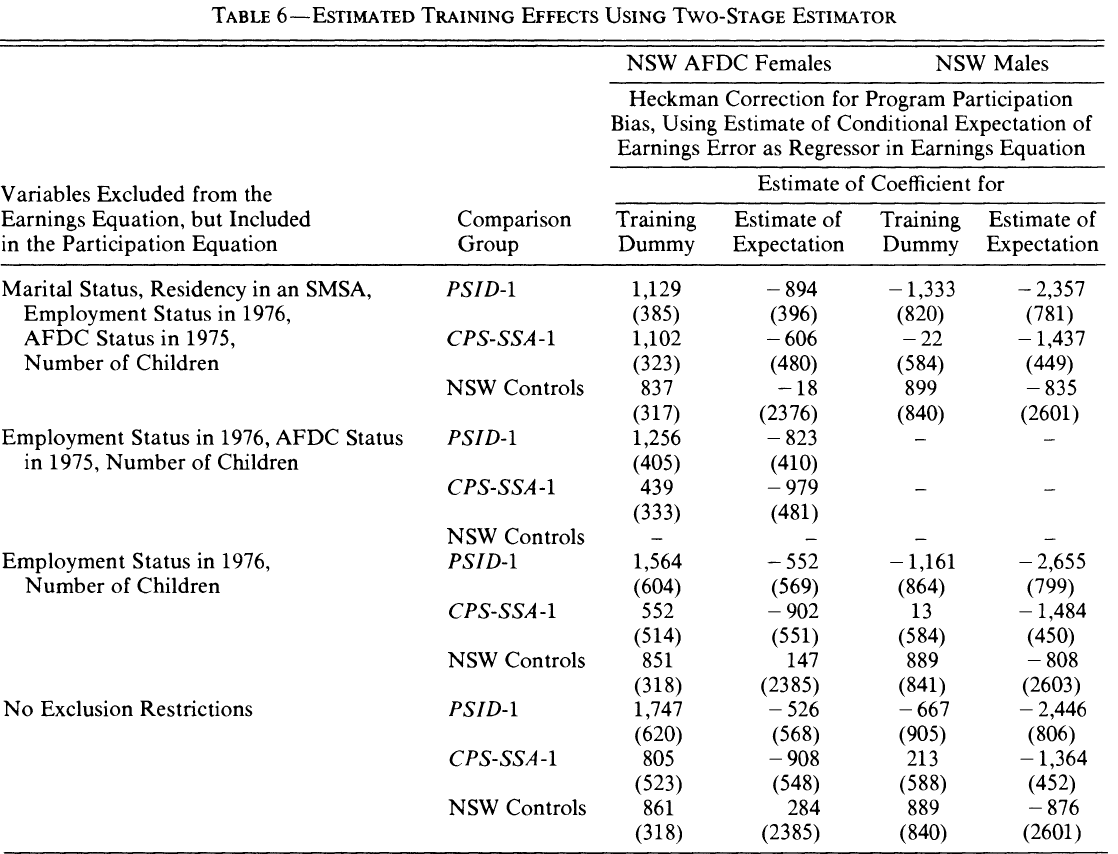
\includegraphics[width=1.0\linewidth]{graphs/lalonde86_6.png}

\end{frame}

\begin{frame}{Heckman correction}
\begin{itemize}
	\item Estimates for women sensitive to the choice of sample and exclusion restriction.
	\item Non-experimental and experimental estimates for men are not even close.
	\item Using better matched control groups results in huge std. errors (not reported in table 6)
\end{itemize}
\end{frame}

%slide 25
\begin{frame}
\frametitle{LaLonde's conclusion}

\begin {itemize}
\item Results are very sensitive to sample specification and econometric method
\item Virtually as many estimates of training effects can be obtained as there are data sets and methods
\item Randomized experiments are necessary to evaluate the causal training effects
\end{itemize}

\end{frame}



%slide 26

\begin{frame}
\frametitle{Dehejia and Wahba JASA (1999)}


\begin{itemize}
	\item Regression based methods cannot recover the experimental extimate (LaLonde 1986)
	\item Are propensity score methods more successful?
\end{itemize}

Problems with NSW training evaluation
\begin{itemize}
	\item Small homogeneous treatment group 
	\item Large, very heterogeneous control groups in non-experimental setting
	\item Big differences in observable characteristics $\rightarrow$ ''limited overlap'' 
	\item Search for the ''best'' subset of the control group to match with treatment group
\end{itemize}


\end{frame}



\begin{frame}
\frametitle{Samples}

\begin{itemize}
	\item Male Participants
	\item Lalonde: training participants in 1976 and 1977: 297T, 425C
	\item Dehejia and Wahba, participants in 1977: 185T, 260C
	\item Additional year of pre-treatment earnings: important control variable
	\item Treatment group from experimental data
	\item Control groups: based on survey data
	\item Replicate Lalonde's results for linear regression and fixed effects
\end{itemize}

\end{frame}

 \frame{ \frametitle{}
\begin{center}
\begin{figure}[t]
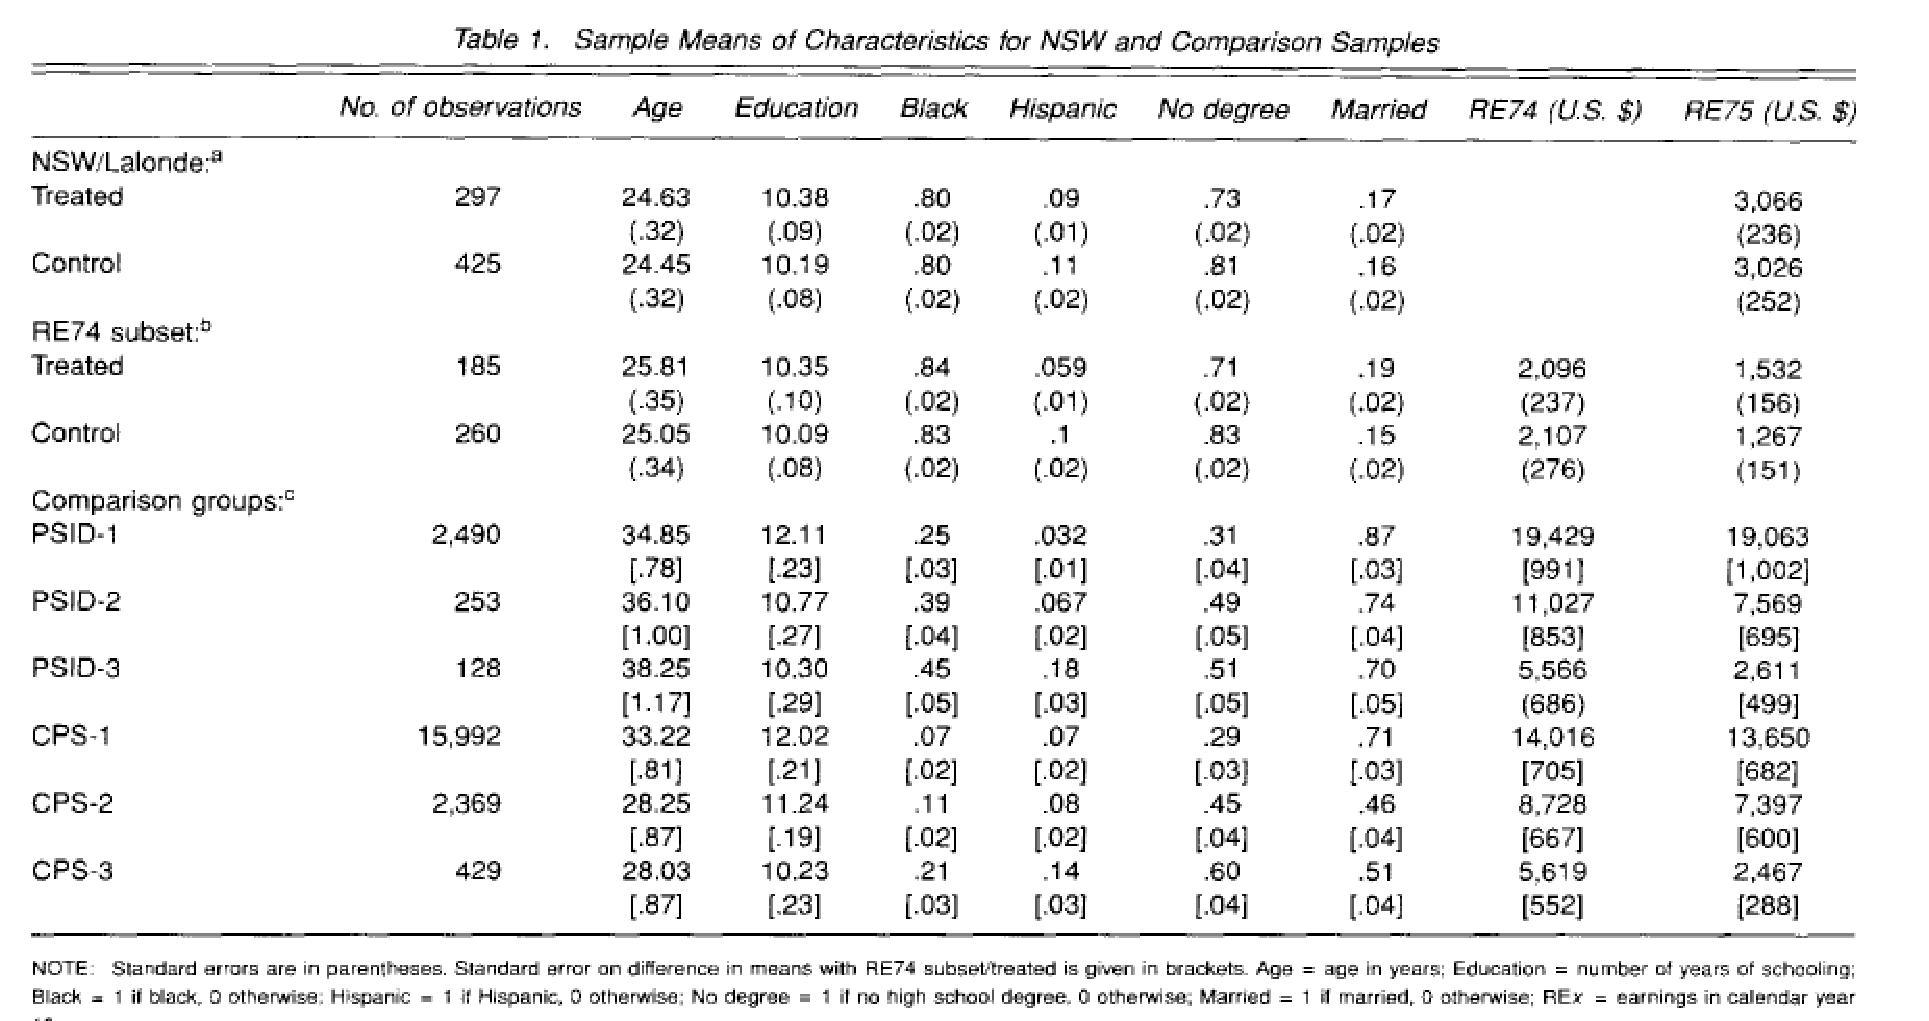
\includegraphics[width=1.0\linewidth]{graphs/dehe_tab1.pdf}
\end{figure}
\end{center}
 }

\begin{frame}
\frametitle{Propensity score methods}

Average treatment effect on the treated
\[
	\delta_{TOT} = E(Y_{1i}|D_i=1)-E(Y_{0i}|D_i=1)
\]
Identification assumption
\[
	(Y_{1i}, Y_{0i}) \amalg D_i|X_i
\]
Conditional Independence Assumption or ''Selection on Observables''
\bigskip

Propensity Score Theorem:
\begin{equation*}
    \{Y_{1i},Y_{0i}\} \amalg D_i|p(X_i)
\end{equation*}
Propensity score $p(X_i)=Prob(D_i=1|X_i)$
\end{frame}

\begin{frame}
\frametitle{Estimation steps}

\begin{enumerate}

	\item Estimate the propensity score $\hat{p}(X)$
	\item Matching on the propensity score
	


\end{enumerate}
	Why $\delta_{TOT}$, not $\delta_{ATE}$? NSW experiment gives $\delta_{TOT}$; we can't use it to say much about the general population.
\end{frame}

\begin{frame}
\frametitle{Estimation of the propensity scores}


\begin{itemize}
  \item Estimate a parsimonious logit for $P(D_i=1|X_i)$
  \item Stratify the data by quintile blocks of $\hat{p}(X_i)$
  \item Compare $\bar{X}_C-\bar{X}_T$ in each block. Use a t-test or F-test of significant differences in means
\begin{enumerate}
  \item if $X_i$ are balanced in each block STOP
  \item if not balanced, divide block in 2 parts and re-evaluate
  \item if $X_i$ not balanced in all blocks re-specify the logit: add interaction terms and polynomials
\end{enumerate}
\end{itemize}
See also:   Caliendo, Marco and Sabine Kopeinig (2008), "Some Practical Guidance for the Implementation of Propensity Score Matching" Journal of Economic Surveys, 22(1), 31-72.	
\end{frame}

\frame{ \frametitle{PSID}
\begin{center}
\begin{figure}[t]
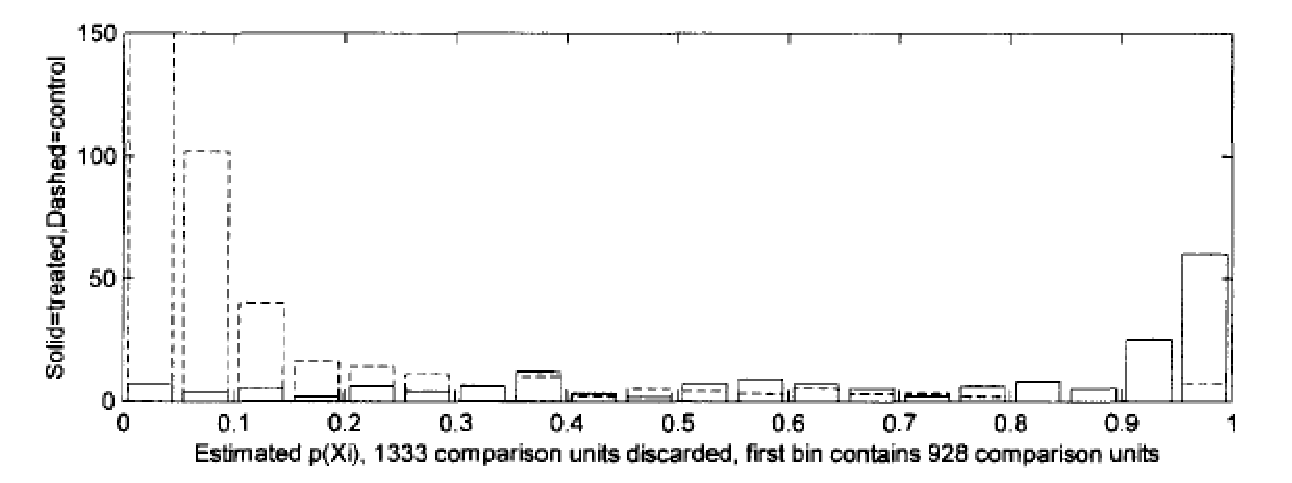
\includegraphics[width=1.1\linewidth]{graphs/dehe_fig1.pdf}
\end{figure}
\end{center}
 }


 \frame{ \frametitle{CPS}
\begin{center}
\begin{figure}[t]
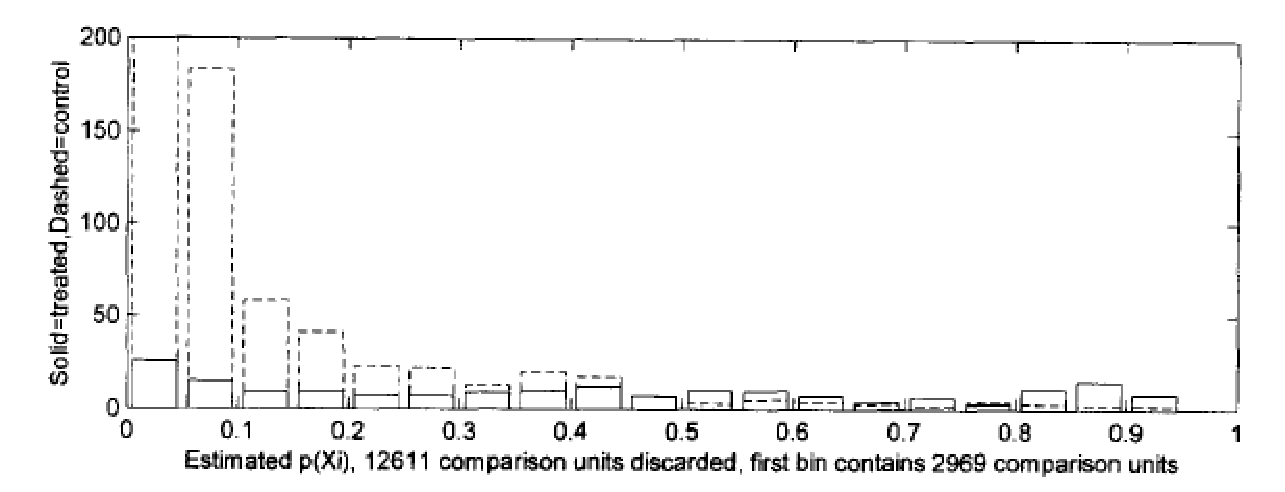
\includegraphics[width=1.1\linewidth]{graphs/dehe_fig2.pdf}
\end{figure}
\end{center}
 }
 
\begin{frame}
\frametitle{Propensity scores}

\begin{itemize}

\item  Limited overlap:
\item  Comparison units are dropped if $\hat{p}_j < min_{D_i=1}\hat{p}_i$, 12,611 dropped from CPS sample, 1333 from PSID sample
\item  Few observations in the control groups with high propensity scores.
\end{itemize} 

\end{frame}

%slide 27

\begin{frame}
\frametitle{Matching Methods}


\begin{itemize}
\item Regression on the propensity score
\begin{eqnarray*}
Y_{it}&=& \delta D_i +  \gamma_1 \hat{p}_{it} +  \gamma_2 \hat{p}^2_{it} +  \epsilon_{it} \;\;\; \text{or}  \\
Y_{it}&=& \delta D_i +  \gamma_1 \hat{p}_{it} +  \gamma_2 \hat{p}^2_{it} +  \beta X_{it}+  \epsilon_{it}
\end{eqnarray*}
\item Stratification: Within block regression
\item Matching on propensity score: find closest match based on the propensity score
	\begin{itemize}
		\item with/without replacement
		\item how many comparison units?
		\item nearest neighbor matching
		\item match within an interval with similar values of the propensity score
	\end{itemize}

\end{itemize}

\end{frame}

\frame{ \frametitle{}
\begin{center}
\begin{figure}[t]
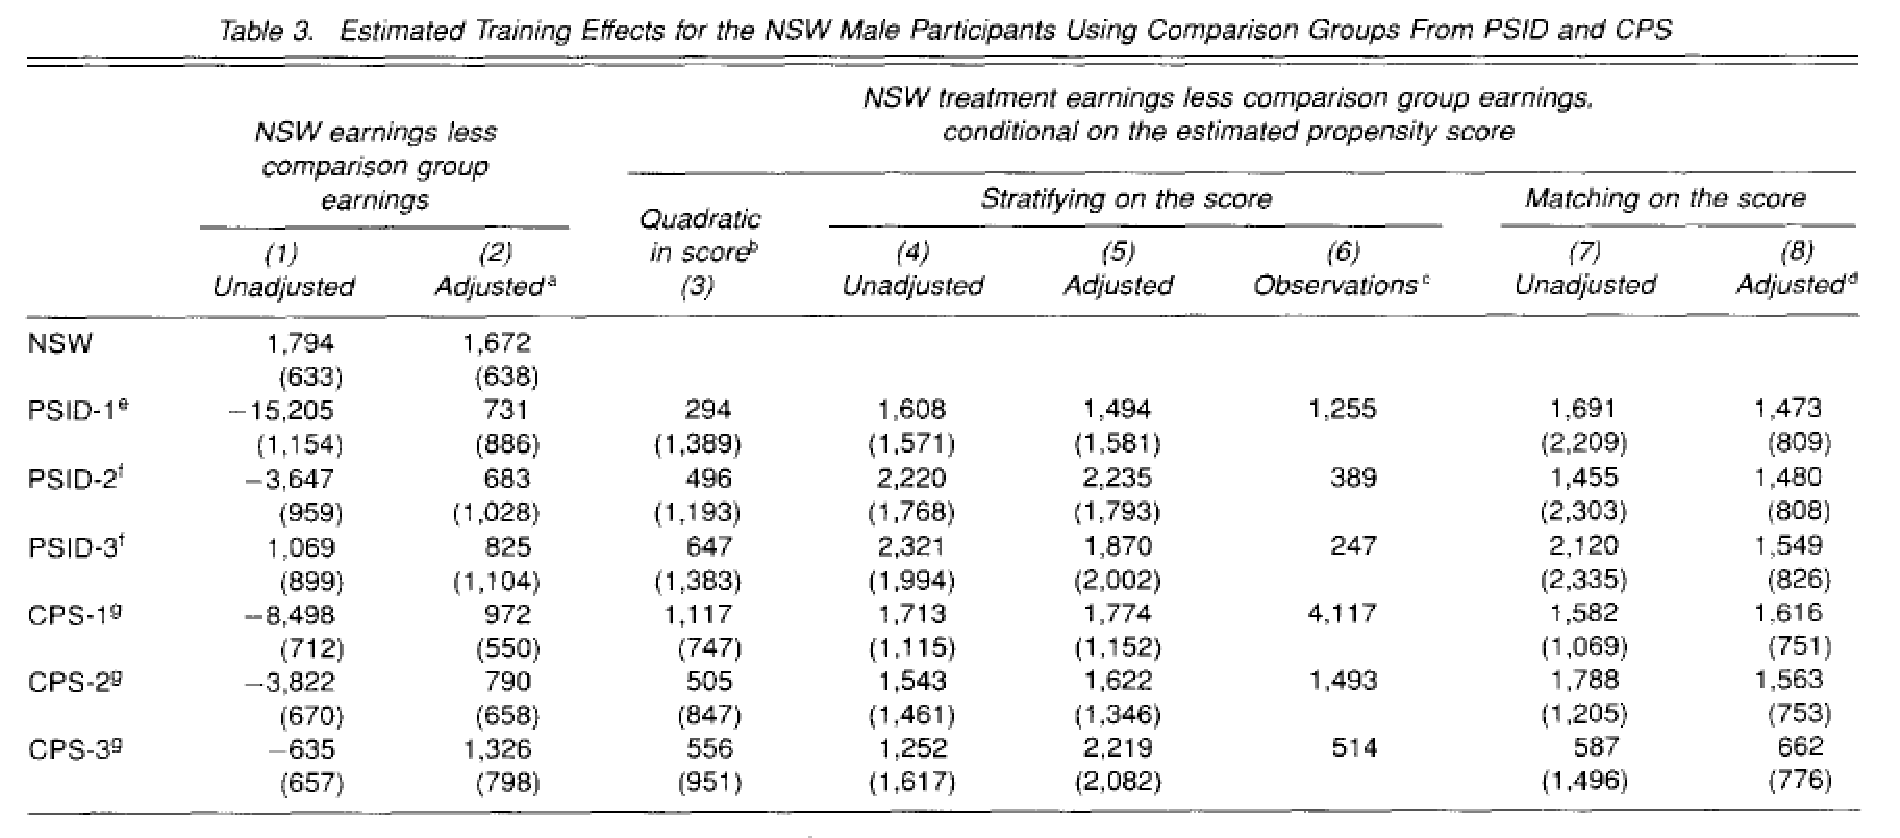
\includegraphics[width=1.0\linewidth]{graphs/dehe_tab3.pdf}
\end{figure}
\end{center}
 }


\frame{ \frametitle{}
\begin{center}
\begin{figure}[t]
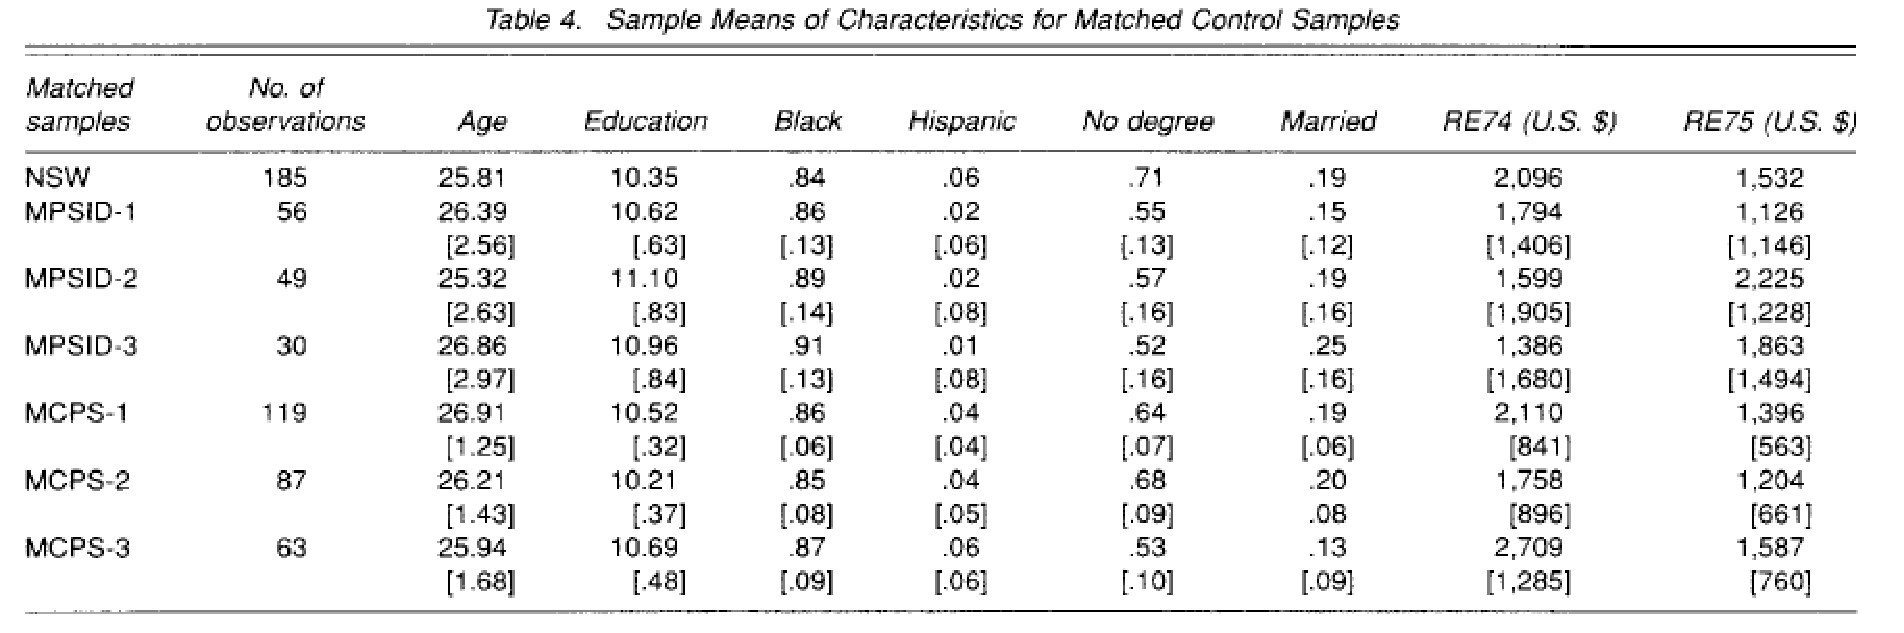
\includegraphics[width=1.0\linewidth]{graphs/dehe_tab4.pdf}
\end{figure}
\end{center}
 }

\frame{ \frametitle{}
\begin{center}
\begin{figure}[t]
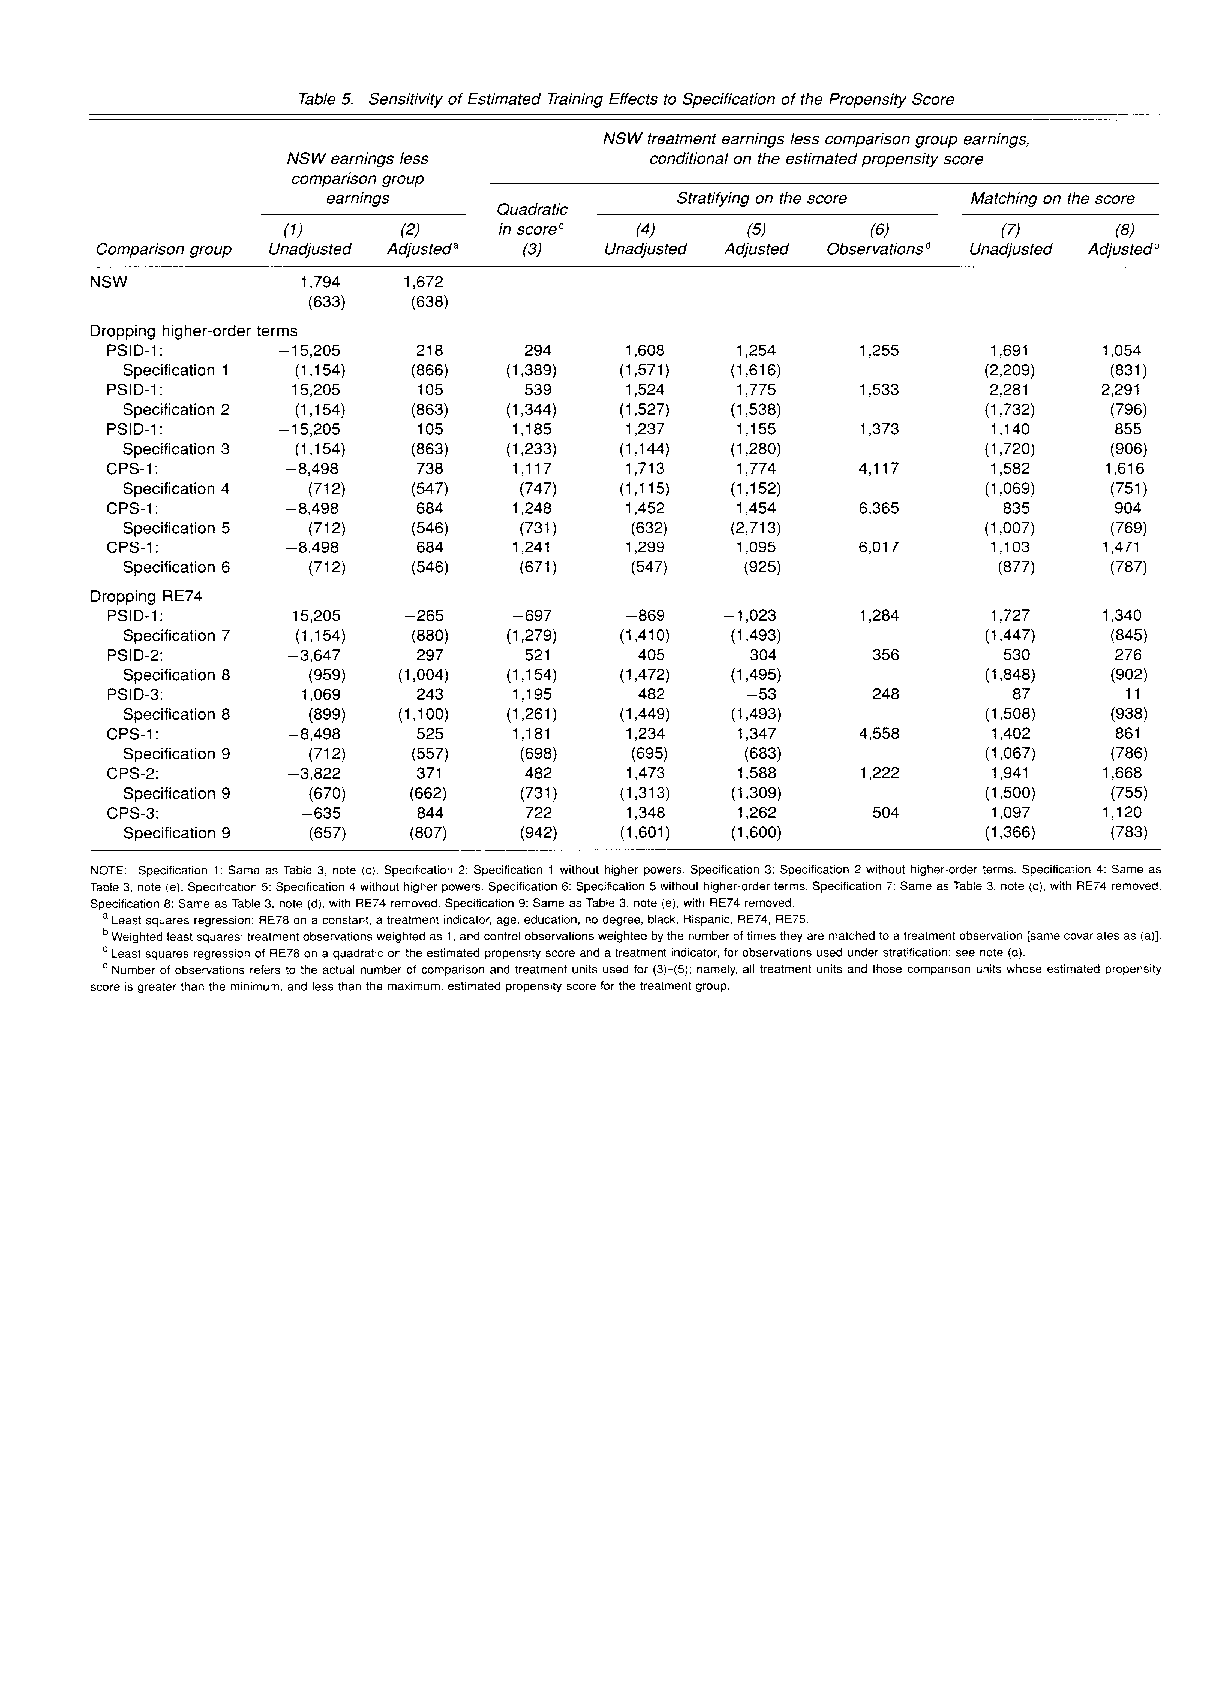
\includegraphics[width=1.0\linewidth]{graphs/dehe_tab5.pdf}
\end{figure}
\end{center}
 }


\begin{frame}
\frametitle{Matching Results}


\begin{itemize}

\item Baseline: experimental results
\item Matching on propensity score works better than quadratic control
\item Creation of ad hoc subsamples of the non-experimental comparision group neither necessary nor desirable (PSID-2, 3, CPS-2, 3).

Don't stratify manually unless you know what you are doing.
\item Sensitivity to specification of p-score --- diagnose p-score issues by comparing treatment and control in terms of $X$ within strata

\end{itemize}

\end{frame}



\end{document}













% slide 20


\begin{frame}
\frametitle{Propensity Score}



\begin{itemize}
\item Slope $m_1$ gives union selection on observables bias in $\bar{Y}_1- \bar{Y}_0$ because $m\neq0$
\item $m_1-m_0$ differential selection in to the 2 groups heteregenous treatment effect.
\item $\hat{p}_1- \hat{p}_0$ fixed $\hat{p}_j$ union wage gap adjusted for selection on $x$
\item ``Unrestricted'' description of selection and heterogeneity in TE
\item Under the initial assumption $\left\{T_i|(Y_{0i}, Y_{1i})\right\}|X$
\end{itemize}
ii) Regression:
\begin{eqnarray*}
	y_i= \alpha+\theta T_i+ \delta_1 \hat{p}_i+ \delta_2 T_i(\hat{p}_i-\mu_p)+ u_i
\end{eqnarray*}
\begin {itemize}
\item $\hat{\mu_p}=\frac{1}{N}\sum \hat{p}_i$
\item $\delta_1 \approx m_0$ and $\delta_2 \approx m_1-m_0$
\item $\delta_1+ \delta_2=m_1$.
\item Linear Specification, Include polynomials in $\hat{p} (X_i)$. Control for $X_i \beta$
\end{itemize}

\end{frame}




%slide 2


\begin{frame}
\frametitle{Matching}
\begin{itemize}
\item Binary treatment $D_{i} =1$ outcome $Y_{i}$ many control variables $X_{i}$ potential outcomes  $Y_{1i},Y_{0i}$
\item CIA $Y_{1i}, Y_{0i} \bot (D_{i} | X_{i})$
\item Linear regression approximates $E[Y_{i} | X_{i}, D_{i}]$
\item Non-linear alternatives?
\begin{eqnarray*}
E[Y_i | X_i, D_i=1]- E[Y_i | X_i, D_i=0]=E[Y_{1i}-Y_{0i} | X_i]
\end{eqnarray*}
\item Estimands of Interest:
\end{itemize}
\begin{eqnarray*}
&& E\left\{E[Y | X_i, D_i=1]- E[Y_i | X_i, D_i=\right\}\\
&=&E\left\{[Y_{1i}-Y_{0i} | X_i]\right\}= E[Y_{1i}-Y_{0i}]=\delta_{ATE}
\end{eqnarray*}

\begin{eqnarray*}
&&E\left\{E[Y_i | X_i, D_i=1]- E[[Y_i | X_i, D_i=0]|D_i=1]\right\}\\	
&=&E\left\{E[Y_{1i}-Y_{0i} | X_i]|D_i=1\right\}\\
&=& E[Y_{1i}-Y_{0i}| D_i]=\delta_{TOT}
\end{eqnarray*}


\end{frame}



% slide 3


\begin{frame}
\frametitle{Matching}
\begin{itemize}
\item Define:

\begin{eqnarray*}
\delta_{x}&=& E[Y_i | X_i, D_i=1]- E[Y_i | X_i, D_i=0]\\
\delta_{TOT}&=&\sum_{x} \delta_x P[X_i=x| D_i=1]\\
\delta_{ATE}&=&\sum_{x} \delta_x P[X_i=x]
\end{eqnarray*}
\item Example:Effect of smoking on Mortality
\begin{itemize}
	\item Compare mortality rates of smokers plus non-smokers
	\item Covariate: Age.
	\item  Mean age of smokers< Mean age of non-smokers.
	\end{itemize}
\end{itemize}
\end{frame}



% slide 4

\begin{frame}
\frametitle{Matching}

\begin{eqnarray*}
X_i= \left\{Age<30, Age 30-40, Age 40-50, Age>50\right\}
\end{eqnarray*}
\begin{figure}[h]
	\centering
		\includegraphics[width=1.00\textwidth]{graphs/table.pdf}
	\label{fig:table}
\end{figure}


\begin{eqnarray*}
\delta_{TOT}&=&(\bar{Y}_{s,30}-\bar{Y}_{N,30})\frac{n S_1}{NS}+ (\bar{Y}_{S,40}-\bar{Y}_{N,40})\frac{n S_2}{NS}+\ldots\\
\delta_{ATE}&=&(\bar{Y}_{s,30}-\bar{Y}_{N,30})\frac{n_1}{N}+\ldots
\end{eqnarray*}

\end{frame}

%slide 4.5

\begin{frame}
\frametitle{Regression-Matching}
\begin{itemize}
\item  Define $d_{ix}=1[X_i=x]$ dummy variable indicating regression
\begin{eqnarray*}
	Y_i= \sum d_{ix} a_x + \delta_R D_i+ e_i\nonumber
\end{eqnarray*}
\item Model Saturated in $X_i$ (fully saturated interaction $D_i \times d_{ix}$)


\item This method generates different weights
\begin{eqnarray*}
	\delta_R&=&\frac{Cov(Y_i, \tilde{D}_i)}{V\tilde{D}_i}=\frac{E[[D_i-E(D_i|X_i)Y_i]]}{E[[D_i-E(D_i|X_i)]^2]}=\cdots\nonumber\\
	        &=& \frac{\sum \delta_x P(D_i=1|X_i=x)(1-P(D_i=1|X_i=x))P(X_i=x)}{\sum  P(D_i=1|X_i=x)(1-P(D_i=1|X_i=x))P(X_i=x)}\nonumber
\end{eqnarray*}
\end{itemize}

\end{frame}


% slide 5

\begin{frame}
\frametitle{Regression-Matching}

\begin {itemize}
\item $\delta_{TOT}$ puts most weight on X-cells where it is most likely to be treated
\item $\delta_{R}$ puts most weights on X-cells where variance of treatment is highest (balance of treated plus controls)
\item Cells where $D=0$ or $D=1$ are not considered
\item ``Common Support'' condition estimates limited to cells where treated plus controls covariate values can be found.
\item Estimators: Problems with manny $X$ variables.
\end {itemize}
\end{frame}






%slide 6

\begin{frame}
\frametitle{Propensity Score}

\begin{eqnarray*}
P(X_i)= E[D_i|X_i]=P[D_i=1|X_i]\nonumber
\end{eqnarray*}
\begin {itemize}
\item \textbf{Propensity Score Theorem}:

Suppose CIA holds, $\left\{Y_{0i}, Y_{1i}\right\} \bot (D_i|X_i)$. Then  $\left\{Y_{0i}, Y_{1i}\right\} \bot (D_i|P(X_i))$

\item \textbf{Proof}:

	\[
	P[D_i=1|Y_{j1}, P(X_i)]= E[D_i|Y_{ji}, P(X_i)]
\]

\begin{eqnarray*}
&= E\left\{E[D_{i}| Y_{ji},  P(X_i), X_i]|Y_{ji}, P(X_i)\right\} \nonumber\\
&=E\left\{E[D_{i}| Y_{ji}, X_i]|Y_{ji}, P(X_i)\right\}\nonumber\\
&=E\left\{E[D_{i}| X_i]|Y_{ji}, P(X_i)\right\} \nonumber\\
&=E\left\{E[  P(X_i]|Y_{ji}, P(X_i)\right\}\nonumber\\
&=P(X_i)\texttt{ does not depend on $Y_{ji}$}\nonumber\\
\end{eqnarray*}

\end{itemize}
\end{frame}






% slide 7

\begin{frame}
\frametitle{Propensity Score}


\begin{eqnarray*}
OVB=  \frac{Cov(Y_i, D_i)}{Var(D_i)}=\rho + \underbrace{\gamma^{'} \delta_{XD_{i}}}_{=0 if  \delta_{XD_{i}}=0}\nonumber
\end{eqnarray*}

\begin {itemize}
\item Need only control for variables correlated with $D_i$
\item Propensity Score Theorem: Need only control for variables affected probability to be treated.
\item Reduced Dimension: Matching on the Propensity Score, 2 Steps:
\begin{itemize}
	\item Estimate Propensity Score
	\item Matching Estimator
\end{itemize}
\item Always start with regression
\item Manny choices when working with Propensity Scores
\begin{itemize}
	\item How to model the score?
	\item How to do inference?
	\item How to specify estimate?
\end{itemize}
\end {itemize}
\end{frame}

%slide 8

\begin{frame}
\frametitle{Selection on Observables}

\begin{itemize}
	\item Assumption:
	\begin{itemize}
	\item  $D_i\bot (Y_{0i}, Y_{1i})| X_i$
	\end {itemize}
	\item Linear Regression:
	
\begin{eqnarray*}
	Y_i= X_i \beta + D_i\theta +u_i\nonumber
\end{eqnarray*}
\begin{itemize}
	\item Condition for $\theta$ constant treatment effect: $E(u_i T_i| X_i\beta)=0$
	\item Restrictions: Functional form, omitted variables.
	\end{itemize}
\item Include non-linear terms
\begin{eqnarray*}
		Y_i= X_i g(X_i) + D_i\theta +u_i\nonumber\\
		E(u_i T_i| g(X_i))=0\nonumber
\end{eqnarray*}

\item General:
\begin{eqnarray*}
D_i\bot(Y_{0i}, Y_{1i}|X_i) \Rightarrow E(u_i T_i| X_i)=0\nonumber
\end{eqnarray*}
\begin {itemize}
\item Arbitrary functional form $g(X_i)$
\item Bias efficiency tradeoff
\end{itemize}
\end{itemize}


\end{frame}


%slide 9


\begin{frame}
\frametitle{Multivariate Matching- Adjustment by Sub-classification}

\textbf{Case Control Method:}
\begin{itemize}
	\item For each treated match control case with identical $X_i$
	\item Problems :
	
	\begin{itemize}
	\item Design Problem if $X_i, T_i$ collinear. Example:
	
	
   \begin{itemize}
	\item $X=0$, not participate;  $X=1$ participate
	\item  $X=0$ some partic.;  $X=1$ partic.
	\item  $X=0$ not participate ;  $X=1$ some partic.
  \end{itemize}
  \item Continious $X_i$ curse of dimensionality.
  \begin {itemize}
  \item Match each treated to one control based on the ``closeness'' of $ X_i$ using some distance metric.
  \item \textbf{Example:} Mortality rates of smokers and non-smokers. Control variable: Age.
  \item Mean age of smokers< Mean age of non-smokers.
  \item Downward Bias: $ \hat{ ATE} = \bar{ Y}_s - \bar{ Y}_N$
	\end{itemize}

	
\end{itemize}
\end{itemize}


\end{frame}




% slide 10

\begin{frame}
\frametitle{Multivariate Matching- Adjustment by Sub-classification}

\begin{itemize}
	\item Idea: Classify by age groups.
	
\begin{figure}[h]
	\centering
		\includegraphics[width=1.00\textwidth]{graphs/table.pdf}
	\label{fig:table}
\end{figure}

\begin{eqnarray*}
	ATE= \frac{n_1}{N} (\bar{Y}_{N,30}- \bar{Y}_{N,30})+ \frac{n_2}{N} (\bar{Y}_{S,40}-\bar{Y}_{N,40})+ \cdots\nonumber
\end{eqnarray*}


\end{itemize}


\end{frame}



% slide 11


\begin{frame}
\frametitle{Multivariate Matching- Adjustment by Sub-classification}
\begin {itemize}

	\item  Many $X$ variables
	
\begin{itemize}
	\item Large number of sub-classes
	\item How can we reduce the dimensionality

	\end {itemize}
\item Propensity Score
\begin{eqnarray*}
	p_i= Pr( D_i=1| X_i)= E(D_i|X_i)= p (X_i)\nonumber
\end{eqnarray*}

\item Propensity Score Theorem

\begin{eqnarray*}
D_i \bot (Y_{0i}, Y_{1i})| X_i \Rightarrow D_i \bot (Y_{0i}, Y_{1i})\bot P(X_i)\nonumber
\end{eqnarray*}

\item If we know $P(X_i)$ we can sub-classify observations along one dimension
\item Match treated and controls with same $P(X_i)$
\item Build sub-groups (e.g. 5 quantiles)
\end {itemize}
\end{frame}

% Slide 12

\begin{frame}
\frametitle{Estimation of the Propensity Score}
	\[
	0\leq Pr(D_i=1| X_i)\leq 1
\]
\begin{itemize}
\item $D_i$ is a binary variable takes values 0 and 1
\item $D_i = X_i\beta + u_i$ linear probability model.
\item $\hat {D}= X_i \hat{\beta}$ can be <0 or >1
\[
	Pr(D_i=1|X_i)=\frac{e^{k(X_i)}}{1+ e^{k(X_i)}}
\]

\item Logit model $k(X)$ ,  flexible functional form.
\item Estimation: Maximum Likelihood.
\item STATA: logit $D, X$, predict $\hat{p}$
\item Aim: Observations with similar $\hat{p}_i$ should have similar $X_i$. Check whether covariates are ``balanced''
\item Application: Rosenbaum + Rubin

\end {itemize}
\end{frame}

%slide 13

\begin{frame}
\frametitle{Algorithm for Estimating Propensity Score}
\begin{enumerate}
	\item Parsimonious Logit
	\item Satisfy data by quantile block of $\hat{p}(X_i)$
	\item Compare $\bar{X}_1-\bar{X}_0$ in each block t-test, (F-test) of significant difference in means.
	
\begin{itemize}
	\item If $X_i$ ``balanced'' in each block stop
	\item Not balanced, divide block in 2 blocks and re-evaluate
	\item If $X_i$  not balanced in all blocks add interactions/polynomials to the logit.
\end{itemize}
\end{enumerate}
\begin{itemize}
	\item Goal: Balance of $X_i$ in treatment plus control group overlap in $\hat{p}_i$ for $D_i=1+D_i=0$
	\item Overlap in $X_i$
	\item Stoppinng Rule: Stop where fail to reject.
	\item $\bar{X}_{1k}= \bar{X}_{0k}$ for > 90\% of all t-tests within block.
\end{itemize}

\end{frame}

 %slide 14

 \begin{frame}
\frametitle{Propensity Score as Diagnostic Tool }
\begin {itemize}
\item Examination of $\hat{p}_{i}$ by $D_i$ gives a sense of ``non-randomness'' of $T_i$ assignment.



\item Observables $X_i$'s very difficult, more likely that unobservable variables also different
\item Box Plot for R.A?
\end {itemize}
\end{frame}




%slide 17

   \begin{frame}
\frametitle{Propensity Score}
\begin{enumerate}
	\item Estimate $\hat{p}(X)$ such that it ``balances'' $X_i$ observations with ``similar'' $\hat{p}(X_i)$ have similar $X_i$.
	
\begin{itemize}
	\item $\bar{X}_{T=1}=\bar{X}_{T=0}$ where $X= (age, income, \cdots)=(X_1\cdots X_k)$
	\item $\bar{X}_{1, T=0}=\bar{X}_{1,T=0}$
	\item Non-random propensity score blocks: $1\cdots J$
	\item $\bar{\hat{P}}_{J,T=1} (X_i)=\bar{\hat{P}}_{J,T=0} (X_i)$ test $\hat{p}$ if $block=j$, by treatment
	\item Show that $X$ balanced in each block.
	
	\[
	\bar{X}_{1, T=0, Block=j}=\bar{X}_{1,T=0, Block=j}
\]
\item t-test $X_1$ if $block=j$, by treatment
\item Box-plot
\end{itemize}
	\item Estimate TE controlling for $\hat{p}(X)$
\end{enumerate}
\end{frame}
% slide 18


   \begin{frame}
\frametitle{Propensity Score}

	
\begin{itemize}
	\item Sub-classification. Estimation of ATE conditional on $\hat{p}_i$
	\item i) Graphical (need manny observations) most general/informative use of $\hat{p}_i$
	
\begin{eqnarray*}
	E(Y_i|D_i=0,\hat{p}_i)&=f_0(\hat{p}_i|T_i=0)\nonumber\\
	E(Y_i|D_i=1,\hat{p}_i)&=f_0(\hat{p}_i|T_i=1)\nonumber
\end{eqnarray*}
\begin{itemize}

	\item Non-parametric estimates useful if $N_c$ and $N_i$ large and satisfy $\hat{p}$ in $m$ quantile blocks $j=1\cdots m$
	\item Example: Union membership and wages, wage gap between union  non union members.
	
\end{itemize}

\end{itemize}

\end{frame}


\frame{ \frametitle{}
\begin{center}
\begin{figure}[t]
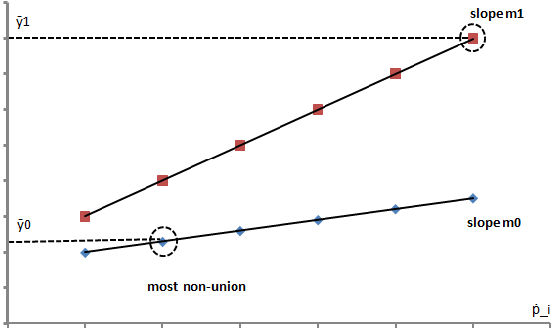
\includegraphics[width=1.0\linewidth]{graphs/grafik.png}
\end{figure}
\end{center}
 }




% slide 20

\begin{frame}
\frametitle{Propensity Score}



\begin{itemize}
\item Slope $m_1$ gives union selection on observables bias in $\bar{Y}_1- \bar{Y}_0$ because $m\neq0$
\item $m_1-m_0$ differential selection in to the 2 groups heteregenous treatment effect.
\item $\hat{p}_1- \hat{p}_0$ fixed $\hat{p}_j$ union wage gap adjusted for selection on $x$
\item ``Unrestricted'' description of selection and heterogeneity in TE
\item Under the initial assumption $\left\{T_i|(Y_{0i}, Y_{1i})\right\}|X$
\end{itemize}
ii) Regression:
\begin{eqnarray*}
	y_i= \alpha+\theta T_i+ \delta_1 \hat{p}_i+ \delta_2 T_i(\hat{p}_i-\mu_p)+ u_i
\end{eqnarray*}
\begin {itemize}
\item $\hat{\mu_p}=\frac{1}{N}\sum \hat{p}_i$
\item $\delta_1 \approx m_0$ and $\delta_2 \approx m_1-m_0$
\item $\delta_1+ \delta_2=m_1$.
\item Linear Specification, Include polynomials in $\hat{p} (X_i)$. Control for $X_i \beta$
\end{itemize}

\end{frame}

%slide 21

\begin{frame}
\frametitle{Propensity Score}
\begin{itemize}
\item iii) Sub-classification
\begin{itemize}
	\item Stratify sample by $\hat{p}_i$ in $j$ blocks

\begin{eqnarray*}
	\hat{\theta}_j &=\bar{Y}_{1j}-\bar{Y}_{0j}\nonumber, or\\
	         Y_{ij}&=\theta_j D_{ij}+ X_{ij}\beta_j +u_{ij}\Rightarrow \hat{\theta}_j\nonumber\\
	\hat{\theta}_j &=\sum ^{j}_{j=1}\frac{\sum_{i\in j}D_i}{N_D}\left(\frac{\sum D_i Y_i}{\sum D_i}- \frac{\sum (1-D_i)Y_i}{\sum (1-D_i)}\right)\nonumber
\end{eqnarray*}

\item (ATE on treated) TOT
\end{itemize}
\end {itemize}
\end{frame}



%slide 22

\begin{frame}
\frametitle{Propensity Score}

\begin{itemize}
\item iv) Use $\hat{p} (x_i)$ as adjustment weights.

\begin{eqnarray*}
\frac{1}{NT} \sum \left(T_i Y_i-(1-T_i)\frac{p(X_i)}{1-P(X_i)}Y_i\right)\nonumber
\end{eqnarray*}
\begin{itemize}
	\item Weighting control observations by $\frac{p(X_i)}{1-P(X_i)}$
	\item Same distribution of $x$ in controls as treated.
	\item Higher $p_i$ more weight
	\item Example: $p(x_i)= 0.2$
	\begin {itemize}
	\item Expect: $\frac{p_i}{1-P_i}=\frac{1}{4}$ controls for every treated observations
	\end{itemize}
	\item More efficient but sensitive to misspecified $\hat {p}_i$
	\begin {itemize}
	\item $\hat{p_i}> p_i$ too much weight
	\item $\hat{p_i}< p_i$ too little
	\end{itemize}
\end{itemize}
\end {itemize}
\end{frame}

%\end{document}


%slide 28





\end {document}

\frame{ \frametitle{Literature}
\begin{itemize}
  \item Rosenbaum, Paul R. and Donald B. Rubin (1984) "Reducing Bias in Observational Studies Using Subclassification on the Propensity Score" Journal of the American Statistical Association, 79, 516-524.
  \item LaLonde, Robert J. (1986), "Evaluating the Econometric Evaluations of Training Programs with Experimental Data", American Economic Review, 76, 604-620.
  \item Ashenfelter, Orley (1987), "The Case for Evaluating Training Programs with Randomized Trials", Economics of Education Review, 6, 333-338.
  \item Dehejia, Rajeev H. and Sadek Wahba (1999) "Causal Effects in Nonexperimental Studies: Reevaluating the Evaluation of Training Programs" Journal of the American Statistical Association, 94, 1053-1062.
  \item Caliendo, Marco and Sabine Kopeinig (2008), "Some Practical Guidance for the Implementation of Propensity Score Matching" Journal of Economic Surveys, 22(1), 31-72.
  \item Imbens, Guido W. (2004) "Nonparametric Estimation of Average Treatment Effects Under Exogeneity: A Review" Review of Economics and Statistics, 86, 4-29.
\end{itemize}
}

\frame{ \frametitle{}
\begin{center}
\begin{figure}[t]
\includegraphics[width=1.0\linewidth]{graphs/lal_tab2.pdf}
\end{figure}
\end{center}
 }







\frame{ \frametitle{}
\begin{center}
\begin{figure}[t]
\includegraphics[width=1.0\linewidth]{graphs/lal_tab5.pdf}
\end{figure}
\end{center}
 }

